\documentclass[11pt,a4paper]{article}
\usepackage[left=2cm,right=2cm,top=2cm,bottom=2cm]{geometry}
\usepackage[utf8]{inputenc}
\usepackage[T1]{fontenc}
\usepackage[english]{babel}
\usepackage{setspace}
\usepackage{parskip}
\usepackage{enumitem} % <--- needed for aligned description lists
\usepackage{hyperref} % for clickable email
\usepackage{mathptmx} 
\usepackage{csquotes}
\usepackage[backend=biber,style=numeric]{biblatex}
\usepackage{titlesec}
\usepackage{tabularx}
\usepackage[table]{xcolor} % Optional: für dezente Hintergrundfarben
\usepackage{booktabs}      % Für schönere Tabellenlinien
\usepackage{longtable}
\usepackage{graphicx}   % wichtig fürs Einfügen von Bildern
\usepackage{caption}    % erlaubt auch unnummerierte Captions (optional)
\usepackage{wrapfig}   % Text um Bilder herum
\usepackage{calc}
\captionsetup[figure]{name=Fig.}
\captionsetup[figure]{aboveskip=1pt, belowskip=-2ex}
\captionsetup[figure]{font={scriptsize,it}} 
\renewcommand*{\bibfont}{\small}  % Schriftgröße der Referenzen
\renewcommand{\arraystretch}{1.2}
\rowcolors{2}{gray!10}{white}
\titlespacing*{\section}{0pt}{0.8ex plus 0.5ex minus .2ex}{0.3ex}
\titlespacing*{\subsection}{0pt}{0.8ex plus 0.5ex minus .2ex}{0.3ex}
\titlespacing*{\subsubsection}{0pt}{0.8ex plus 0.5ex minus .2ex}{0.3ex}
\titleformat{\paragraph}[block]{\normalfont\normalsize\bfseries}{\theparagraph}{1em}{}
\titlespacing*{\paragraph}{0pt}{0.5ex plus 0.2ex minus 0.1ex}{1ex}
\setlist[itemize]{leftmargin=*, topsep=-3pt, itemsep=0pt}
\setstretch{1}

\addbibresource{Daimler.bib}

\begin{document}

\subsection*{Applicant} 
\vspace{1ex}
\textbf{PD Dr. Susanne Weis}\\
Group Leader "Brain Variability", Institute of Neuroscience and Medicine, Brain and Behaviour (INM-7), Research Centre Jülich, Jülich, Germany and \\
Institute of Systems Neuroscience, Medical Faculty, Heinrich Heine University Düsseldorf, Düsseldorf, Germany. \\
\textbf{Contact Details:} eMail: S.Weis@fz-juelich.de, phone: +49 2461 61 85925\\

\subsection*{Scientists and Institutions involved in the research project}
\vspace{1ex}
\textbf{Prof. Dr. Simon Eickhoff}\\
Institute of Neuroscience and Medicine, Brain and Behaviour (INM-7), Research Centre Jülich, Jülich, Germany and \\
Institute of Systems Neuroscience, Medical Faculty, Heinrich Heine University Düsseldorf, Düsseldorf, Germany. 

\textbf{Institute of Neuroscience and Medicine, Brain and Behaviour (INM-7) Research Centre Jülich, 
Jülich, Germany}\\
The proposed work is embedded in a multidisciplinary working team combining knowledge in the field of neuropsychology, structural and functional MRI analysis, 
computational neuroscience and machine learning. 


\newpage

\section*{\Large\textbf{Dynamic Cognition: Movies as a Window into Sex Differences in the Brain}}
\hfill

\subsection*{Project Description} 
\subsection*{Background and Research Question} 

Functional brain imaging, especially fMRI, has been widely used to investigate sex differences in the brain. 
Understanding sex differences in brain function is not only of fundamental scientific interest but also of high societal importance. 
Women and men differ in the prevalence, course, and treatment response of many psychiatric and neurological disorders \parencite{cahillWhySexMatters2006,gobinathSexHormonesGenotype2017}, 
yet current diagnostic and therapeutic strategies rarely account for these differences. By uncovering sex-specific neural mechanisms 
in ecologically valid contexts, this project has the potential to improve diagnostic precision, inform personalized treatments, 
and guide the development of sex-sensitive strategies in medicine, education, and mental health. 
In this way, the proposed work directly addresses the call's emphasis on both scientific originality and societal relevance.\\
We suggest novel brain imaging methodology utilizing naturalistic viewing (NV), i.e. watching movie 
clips in the scanner, for providing new perspectives on sex differences in brain function. While it is common knowledge 
that women and men often react differently to films, our study moves beyond stereotypes (“women prefer emotions, 
men prefer action”) to examine in detail how brain activity and functional connectivity (FC) differ when 
viewing diverse scenes. For example, women may process subtle social cues in dialogue in more depth, whereas 
men may respond more strongly to visual foreshadowing of danger. Through the novel use of NV fMRI, we aim to uncover 
sex-specific neural mechanisms that have remained invisible to traditional approaches, advancing the field far beyond 
the current state of research.\\
Classical studies used task-based (TB) fMRI to provide domain-specific insights into cognitive sex differences 
\parencite{thimmMenstrualCycleEffects2014a,weisDynamicChangesFunctional2011,weisEstradiolModulatesFunctional2008}, 
but with very low ecological validity. More recently, resting-state (RS) fMRI has become the method of choice
for studying sex differences, where data are acquired while subjects relax in the scanner without any specific task 
demand or sensory stimulation. Early RS studies examined group differences in FC patterns between women and men. 
More recently, machine learning (ML) methods have been applied to move beyond group averages: 
sex classification approaches use RS data to predict the sex of individual subjects 
\begin{wrapfigure}{r}{0.3\textwidth} % r = rechts, l = links
  \vspace{-10pt} % optional: kleine Korrektur, damit es bündig startet
  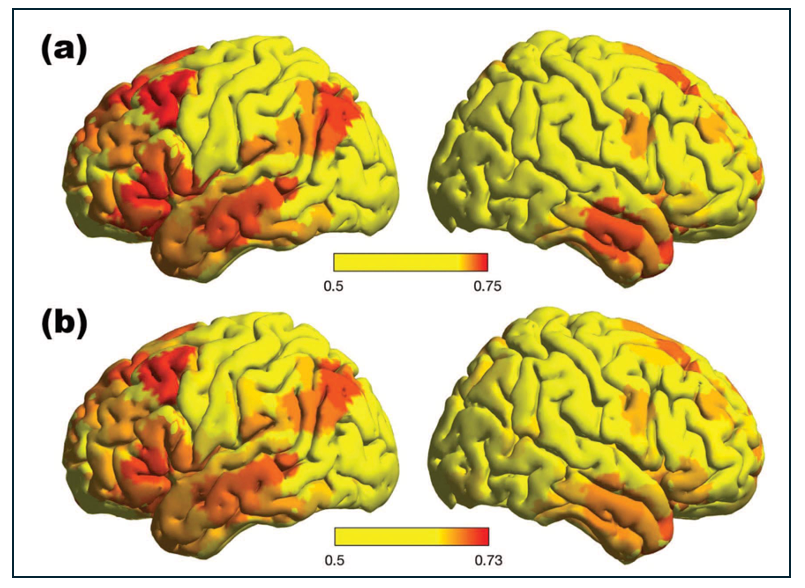
\includegraphics[width=\linewidth]{sex_classification.png}
  \caption{ROI-based sex classification shows high accuracies for (a) within sample CV and (b) across sample classification.}
  \label{fig:sexclass}
\end{wrapfigure}
based on their FC patterns and then infer which brain networks contribute most to distinguishing females from males.
Our own ML work (Fig. 1) identified most predictive brain networks in higher-level regions 
for language, social cognition, and emotion processing \parencite{weisSexClassificationResting2020a,wierschAccurateSexPrediction2023a,wierschSexDifferencesBrain2021a}.\\
However, RS primarily reflects intrinsic, trait-like brain organization. What remains largely unexplored are 
sex differences in the “brain in action” when engaging with complex, multimodal input resembling real life.\\ 
Therefore, the present proposal aims to contribute to closing this gap in knowledge by applying the newly 
emerging NV approach to examine sex-specific brain responses in ecologically valid contexts. 
NV focuses on cognitive processes in dynamic, time-extended, naturalistic contexts, much more akin to
situations which the brain must deal with in real life.
Importantly, as opposed to RS, all participants are exposed to the same stimulus, 
for which content and timing 
is known and can be used in the analyses.
\par\vspace{-\parskip}\noindent % small, controlled separation
NV offers complex, dynamic, and ongoing stimulation similar to experiences in everyday life, 
where low-level (audiovisual) and high-level (cognitive and emotional) content vary fluidly, 
creating a multimodal immersive experience \parencite{sonkusareNaturalisticStimuliNeuroscience2019}. 
This provides the opportunity to capture dynamic neural processing in ecologically valid contexts 
\parencite{vanderwalMoviesMagnetNaturalistic2019} and has been shown to enhance reliability and identifiability 
over RS \parencite{krollNaturalisticViewingIncreases2023}.\\
Our lab has pioneered NV analyses. We developed the \textbf{"Topography-based Predictive Framework" (TOPF)}
\parencite{liTopographybasedPredictiveFramework2023a}, which extracts individual-specific evoked 
topographies and links them to behavior using ML.
\textbf{TOPF} achieved sex classification accuracies of up to 80\% \parencite{liStimulusSelectionInfluences2025a}, 
with key predictive regions associated with emotion, language, and higher cognition, demonstrating the potential of NV to 
reveal novel sex differences.\\
Surprisingly, to our knowledge, no study has yet used NV to systematically examine sex differences. 
In a previous publication \parencite{eickhoffClinicalApplicationsMovie2020a}, we have compared the potential of 
movies for the study of individual brain differences to a cardiac stress-test, 
i.e. to potentially provide a standardized way to study the whole organ while it works to compare function 
across different levels of intensity and demands. 
We therefore expect NV to expose sex differences across a wide range of real-life-like situations — social interactions, 
face and emotion perception \parencite{sonkusareNaturalisticStimuliNeuroscience2019}, 
or complex narratives - that RS approaches cannot capture. Careful stimulus annotation will further allow us to identify the 
specific features and networks driving these differences.
Using advanced neuroimaging and analysis methods, we aim to detect subtle but meaningful sex-related differences 
in brain activity and FC, that can inform our understanding of 
broader cognitive and behavioral differences between females and males.\\
To do so, we will first study FC patterns that are aggregated across the full duration of several minutes of movie watching. 
Then, we will zoom in to
identify specific events that trigger differences between women and men, and finally examine how differences in brain activity
unfold over time and in relation to the progressing content of the movies.\\
This multi-layered approach — combining aggregated and time-resolved FC, network dynamics, and brain activity — offers 
a rich view of sex differences in brain function in ecologically valid settings. 
Results from the proposed project can shed new light on why cognitive and behavioral patterns differ 
between women and men, and why certain neurological and psychiatric disorders present differently across the sexes. 
Such knowledge may improve diagnostic precision and personalized treatments, and support sex-specific 
strategies in healthcare and education.\\
We are uniquely positioned to realize this project, as our lab has already acquired the \textbf{Ju-MOVIES dataset}, 
a rich NV fMRI resource with over 130 participants. It combines extended movie stimuli, 
hormone measures, and detailed scene annotations, providing an unparalleled foundation for 
uncovering sex differences in the brain.\\
For clarity, throughout this proposal “sex” refers to self-reported biological sex. 
We acknowledge that “gender identity”, i.e. the 
subjective identification of an individual as female, male, or one of the other gender identities which might 
be also fluid, also plays a significant role, but this lies 
beyond the scope of the present project.

\subsection*{Data: The Ju-MOVIES dataset}
The proposed work builds on the \textbf{Ju-MOVIES dataset}, which has already been acquired and is 
uniquely suited for investigating sex differences with a NV approach. Its richness and design make it an ideal 
foundation for the present project, which will be further expanded over the course of the proposed project. 
The paradigm comprises seven Hollywood movie excerpts (8 - 10 minutes each) selected to capture diverse social 
interactions, complex situations, and evolving emotions (from “Dirty Dancing”, “Scream”, “Dead Poets Society”, “Forrest Gump”, 
“Dead Man Walking”, “Life is Beautiful”, “The Good, the Bad, the Ugly”), as well as 12 shorter clips and two 
RS scans of about 9 minutes.
Stimuli were chosen to be long enough for participants to grasp the context and empathize with characters, 
ensuring ecological validity.\\
So far, data from 135 healthy participants (68 males, 18 - 35 years) have been collected using state-of-the-art fMRI parameters. 
Alongside fMRI and structural imaging, saliva samples were collected and analyzed for levels of cortisol, estradiol, progesterone 
and testosterone to account for variability related to
\begin{wrapfigure}{r}{0.27\textwidth} % r = rechts, l = links
  \vspace{-10pt} % optional: kleine Korrektur, damit es bündig startet
  \includegraphics[width=\linewidth]{emotions_DMW_edited.png}
  \caption{Exemplary emotion annotation for one of the movie stimuli..}
  \label{fig:dmw}
\end{wrapfigure}
fluctuating hormone levels. 
Oral contraceptive use was documented in women.\\
The movies are richly annotated: 
emotion ratings from 44 additional participants (23 males, age 20-30 years)
for the six basic emotions (happiness, fear, surprise, sadness, disgust and anger \parencite{ekmanConstantsCulturesFace1971a}), 
sampled at 10 Hz confirmed that the stimuli evoke a wide spectrum of affective states (Fig. 2). 
Further annotations by two independent raters include scene content: faces, bodies, male / female presenting characters, ethnicity of characters, presence of children, 
adults, crowds, hands, buildings, vehicles, food, landscapes, animals, plants, movement, social interactions, 
place (inside or outside / urban vs. non-urban), time of day (day or night), weather, presence of music and 
camera movements, enabling fine-grained mapping of movie features to neural responses.
Altogether, Ju-MOVIES offers a rare combination of naturalistic stimulation, hormone measures, 
and detailed scene-level annotations, providing an exceptionally strong basis for the proposed project.

\subsection*{Work Program and Research Methods}
The overarching goal of the proposed project is to augment existing research on sex differences in the brain by 
applying a NV approach. Unlike traditional methods, NV allows for the study of brain responses to complex, dynamically 
evolving situations — much closer to the demands the brain faces in everyday life. With this approach, we aim to move 
beyond the insights gained from RS studies and provide novel perspectives.\\
More concretely, we will first identify which complex situations portrayed in the movie stimuli give rise to the most 
pronounced sex differences. We will then trace these effects to specific narrative events and assess how female and male 
brains respond to them differently.
By combining analyses of temporally aggregated FC, event-related responses, network dynamics, and brain activity, 
this innovative approach will deliver important new insights into the multi-faceted spectrum of sex differences in the brain “in action.”\\

\subsection*{WP 1: Beyond Resting State - Sustained Action States in Naturalistic Viewing}

\textbf{Aim:} \textit{\textbf{WP1} will extend existing RS findings by examining sustained, content-driven brain "action states" 
during NV over several-minute time windows. Using a temporally aggregated FC approach, as commonly applied in RS research, 
we will identify sex differences in these states, map the networks that support them, and compare their predictive power 
against RS connectivity.}

\textbf{Open Question:} \textit{Do sex-specific movie feature networks differ systematically, and if so, 
what do these differences reveal about distinct cognitive strategies in women and men?}

RS studies have demonstrated that sex can be classified with high accuracy based on FC patterns that are 
aggregated across time \parencite{casanovaCombiningGraphMachine2012a,ritchieSexDifferencesAdult2018,weisSexClassificationResting2020a,wierschAccurateSexPrediction2023a,wierschSexDifferencesBrain2021a}. 
Because RS measures brain activity in the absence of external stimulation and any specific tasks, these connectivity patterns are 
typically interpreted as indicators of intrinsic brain organization—capturing stable, trait-like characteristics 
rather than momentary states.\\
In this \textbf{WP}, we go beyond RS by studying sustained FC patterns evoked by complex movie narratives. 
Unlike RS, these naturalistic viewing action states (NV-AS) are driven by the actual content of the films, 
meaning that the brain's functional organization adapts to what happens on screen. Since the content is precisely 
defined and the timing is identical for all participants, we can directly link FC patterns to narrative features and identify
sex-specific differences in relation to the content of the movies.\\
This \textbf{WP} will therefore provide insights into which kinds of complex, 
real-life-like situations give rise to the most pronounced sex differences in brain networks. 
By focusing on the brain "in action", we aim to capture sex differences in the holistic experience of complex situations — an 
approach that goes far beyond RS studies, which mainly reflect intrinsic organization during unconstrained thought. 
NV provides the unique opportunity to study these differences under conditions that mirror real-life cognitive 
and emotional demands, revealing patterns that remain hidden in traditional paradigms.
In line with this, we hypothesize that putting the brain into action will highlight sex differences more strongly 
than the unconstrained state of mind wandering \parencite{vanderwalIndividualDifferencesFunctional2017}.\\
From a methodological perspective, we will build on and extend our previously developed sex classification 
framework \parencite{weisSexClassificationResting2020a}. Specifically, fMRI data will be divided 
into non-overlapping brain regions using an established parcellation \parencite{schaeferLocalGlobalParcellationHuman2018}. 
For each region, a representative time course will be extracted, and FC with all other regions will be calculated. 
These connectivity patterns will then serve as input features for sex classification using a cross-validation (CV) approach, 
resulting in a spatial map of classification accuracies (c.f. Fig. 1) for both RS and each NV-AS (i.e., each movie).
Importantly, and in contrast to most previous studies, we will explicitly incorporate hormone levels and oral contraceptive (OC) 
status in women as confounding variables in all prediction analyses. This ensures that the observed effects truly reflect 
sex differences rather than hormone-related variability. In addition, we will implement rigorous measures to avoid 
“confound leakage” \parencite{hamdanConfoundleakageConfoundRemoval2022a}, which can otherwise bias results. 
Taken together, these methodological precautions will guarantee robust, reliable, and unbiased findings.

\subsubsection*{WP 1.1:  Comparing sex classification accuracies between RS and NV-ASs}
As a first step, we will compare sex classification performance between RS and NV-AS (averaged across all movies) within each brain region, 
using corrected resampled \textit{t}-tests \parencite{nadeauInferenceGeneralizationError2003a}. 
If classification accuracies are higher during NV-AS than during RS, this would indicate that sex differences 
become more pronounced when the brain is “in action” rather than at rest.\\
Beyond overall accuracy, we will examine the spatial distribution of brain regions that are most discriminative in NV-AS, 
thereby highlighting the brain networks that drive these differences. To better interpret their functional relevance, 
the identified networks will be characterized using functional decoding \parencite{foxMetaanalysisHumanNeuroimaging2014a}.\\
Previous RS studies have often reported sex differences in the default mode network (DMN) 
\parencite{weisSexClassificationResting2020a,zhangFunctionalConnectivityPredicts2018}. 
For NV-AS, however, we expect to observe effects in higher-order cognitive or task-general networks 
\parencite{hugdahlExistenceGeneralizedNonspecific2015a}. Moreover, we hypothesize that sex classification based on 
NV-AS will outperform RS, in line with findings for other 
phenotypes \parencite{finnCanBrainState2017a,vanderwalIndividualDifferencesFunctional2017} and with recent 
evidence that NV improves individual identifiability compared to RS \parencite{krollNaturalisticViewingIncreases2023}.

\subsubsection*{WP 1.2: Which movie features drive sex classification accuracies?}
To investigate which types of complex situations maximize sex differences in the brain, we will characterize each movie clip by a 
comprehensive set of visual and auditory features across its entire duration. These will include low-level 
properties such as mean motion energy, visual brightness, and auditory loudness, as well as higher-level properties such as the 
number of faces, social interactions, and spoken words. Many of these features can be automatically 
extracted \parencite{mcnamaraDevelopingComprehensiveFramework2017a,radfordRobustSpeechRecognition2022}, while others will come 
from our detailed manual annotations.\\
Next, we will apply a multiple regression approach to compare sex classification accuracies across the whole brain between 
different movie clips. This analysis will identify which movie features are most predictive for classification performance within 
each brain region. Because higher accuracy reflects stronger sex differences, this procedure will reveal which specific 
features of the movies evoke the most pronounced differences.\\
By clustering brain regions according to their feature profiles, we will uncover brain networks in which sex differences are jointly 
driven by particular features. We hypothesize that some of these networks will map onto well-established cognitive domains such as 
language or spatial cognition \parencite{halpernSexDifferencesCognitive2000a,kimuraSexCognition2000a}, while others will 
reflect more generalized, task-independent resources \parencite{hugdahlExistenceGeneralizedNonspecific2015a}. 
We expect that domain-specific networks will generally achieve higher classification accuracies than domain-general ones.\\
Finally, in an exploratory step, we will compare how the identified networks are expressed differentially n women and men. 
By summarizing each network's connectivity pattern separately for females and males (by use of a principle component analysis, PCA), we 
will derive "typical" network signatures
for each movie feature cluster. This will help us identify sex-specific cognitive strategies for processing complex, 
real-life-like situations.

\subsection*{WP 2: Going dynamic: Sex differences in time-resolved FC}

\textbf{Aim:} \textit{\textbf{WP2} will build on \textbf{WP1} by applying a time-resolved FC approach to detect specific narrative events 
that trigger sex differences during the experience of complex situations. Leveraging detailed annotations of the movie content,
we will determine which types of scenes produce the strongest sex differences and reveal sex-specific cognitive strategies 
for processing them.}

\textbf{Open Questions:} \textit{How do naturalistic sex differences observed here relate to findings 
from traditional paradigms (e.g., isolated face viewing)? Do the same brain regions emerge, 
or do new networks appear under ecologically valid conditions?}  

While \textbf{WP1} investigates sex differences in sustained “action states” evoked by movies, 
\textbf{WP2} makes use of one of the main strengths of NV: its continuous and dynamic variation in content. 
Rather than looking only at averages across longer time windows, this WP aims to zoom in on how the brain responds 
to specific moments in the unfolding story. 
Because all participants are exposed to the same time-locked stimulus, we can examine the effect of the movie 
content on the brain directly and with high temporal precision. This allows us to go beyond asking whether women and 
men differ in processing complex situations \textit{on average}, and instead pinpoint exactly \textit{which moments} in the 
evolving narrative trigger sex-specific brain network configurations. 
In other words, this WP shifts the focus from \textit{what kinds of situations} \textbf{(WP1)} to 
\textit{when and how} sex differences manifest during real-life-like experiences.\\
Methodologically, fMRI data will again be divided into brain regions, and region-wise time courses 
will be used to calculate moment-by-moment co-fluctuations between regions using the \textbf{edge time series (eTS)} 
approach \parencite{betzelLivingEdgeNetwork2023,faskowitzEdgecentricFunctionalNetwork2020a}. 
This method effectively “unwraps” FC into its temporal development, producing a time series of co-fluctuation magnitudes 
for each connection between brain regions.\\
To identify dynamic FC differences between women and men during movie watching, we will focus on time points where 
their connectivity patterns diverge most strongly. To identify such time points, a ML classifier will be trained for each
time point to distinguish female from male FC patterns. Because the number of connections between all brain regions is extremely high, 
dimensionality will first be reduced using a PCA approach. A certain number of components (e.g. the first 50) 
will then be used as classifier features, and classification accuracy will be determined via CV. Hormone levels and OC status will be
included as confounds to ensure that detected effects truly reflect 
sex differences, and possible confound leakage \parencite{hamdanConfoundleakageConfoundRemoval2022a} will be controlled for.\\
Significant time points, i.e. those where classification accuracy is reliably above chance (p < 0.05, permutation test), 
will be treated as markers of narrative events that evoke the strongest sex differences. To understand what drives these effects, 
each of these events will be described in detail using our movie annotations, including both discrete features 
(e.g. the presence of faces, bodies, animals, or scene cuts) and continuous ones (e.g. brightness, 
sound intensity, or background music). By combining all of these descriptors, we will identify a 
set of movie features that captures the key visual and auditory elements present in the movie at those moments which 
elicit most pronounced sex differences.
Next, we will group (cluster) the significant time points from all movies based on their annotated features, allowing us to 
identify categories of scenes that consistently give rise to sex-specific differences. For each category, we will then 
derive typical female and male FC patterns using a PCA approach and apply thresholds to highlight the most discriminative brain regions 
and connections. In this way, we can identify the brain networks that respond differently in women and men to specific 
types of naturalistic events.\\
Altogether, \textbf{WP2} will reveal which narrative elements most strongly drive sex differences in time-resolved FC and how 
these differences are expressed across brain networks. Some of these patterns are expected to overlap with domains already 
identified in classical studies (e.g., sex differences in face perception). However, by taking advantage of naturalistic, dynamic stimuli, 
this WP will provide a far richer and ecologically valid picture — capturing sex-specific cognitive strategies for dealing with 
complex, multimodal real-life-like situations. These sex-specific brain network patterns may shed new light on the 
different strategies women and men use when navigating complex emotional and social events.

\subsection*{WP 3: Shared but Unique: Examining Sex-Specific Responses to Dynamic Emotions}

\textbf{Aim:} \textit{\textbf{WP3} will shift the focus from connectivity to brain activation patterns, examining how typical 
female and male responses emerge across brain regions during evolving movie narratives. This analysis will enrich \textbf{WP1} 
and \textbf{WP2}  by characterizing how women's and men's brains differ in their regional activation patterns, 
thereby complementing the connectivity-based findings.}

\textbf{Open Questions:} \textit{Which brain regions display distinct time-resolved responses to emotional content in 
women and men, and are these effects stable across movie narratives? Do particular emotions (e.g., fear, anger, happiness) 
disproportionately trigger divergent neural activity between the sexes?}

A major advantage of NV paradigms over RS is that all participants are exposed to the same stimulus, 
producing synchronized neural responses across individuals, while still preserving meaningful inter-individual 
differences \parencite{finnIdiosynchronySharedResponses2020a,vanderwalIndividualDifferencesFunctional2017}. 
This \textbf{WP} capitalizes on that property to focus directly on the evolution of neural activation patterns 
during movie watching, asking whether and how females' and males' brains differ in their responses 
to dynamic, emotionally rich content. Since movies are especially effective in eliciting 
strong emotions \parencite{grossEmotionElicitationUsing1995,westermannRelativeEffectivenessValidity1996}, 
and sex differences in emotion perception and regulation are well documented 
\parencite{domesNeuralCorrelatesSex2010a,gardenerSexDifferencesEmotion2013a}, 
we focus here on differences in emotional brain responses unfolding over naturalistic narratives. 
This extends prior work that typically examined only isolated emotions in artificial tasks.\\  
Methodologically, we will employ the \textbf{Topography-based Predictive Framework (TOPF)} recently 
developed in our lab \parencite{liTopographybasedPredictiveFramework2023a}. For each brain region, 
TOPF extracts the shared time course of brain responses across participants (via PCA) and quantifies how 
strongly each individual expresses this response. In the present context, we will compute separate 
shared response time courses for women and men, while regressing out hormone levels to ensure that 
results reflect sex differences rather than hormone-driven variability.\\ 
Analyses will proceed in two steps. Firstly, we will directly compare the typical female and male time courses 
for each brain region to identify regions where the evoked responses fundamentally diverge between sexes. 
To probe whether such differences are driven by emotions depicted in the movies, we will correlate the 
sex-specific shared response with existing emotion annotations (six basic emotions). 
High correlations with particular emotions (e.g., fear, happiness) will reveal which emotions most 
strongly drive sex differences.\\
Second, for regions where overall time courses do not differ significantly, we will test whether the \textit{intensity} of 
response expression differs between the sexes using two-sample \textit{t}-tests, identifying regions in which 
females and males process the narrative similarly in form but differently in strength. 
Such regions are expected mainly in higher-order cognitive areas, and functional decoding will be
used to interpret their domain-specific relevance \parencite{foxMetaanalysisHumanNeuroimaging2014a}.\\  
Finally, we will assess whether whole-brain patterns reveal sex-typical processing of dynamic narratives. 
For each subject, we will compute the similarity of their brain response to the sex-specific shared response 
across all regions, and classify subjects accordingly. High classification accuracy would indicate 
the existence of typical female and male whole-brain response patterns; failure to classify would 
suggest that individual variability outweighs sex as the organizing principle.\\
Altogether, \textbf{WP3} will identify sex-specific regional and whole-brain patterns in the perception of 
dynamic emotions, providing novel insights into how women and men process emotionally charged, 
real-life-like situations.\\  
[6pt]
In sum, by combining novel NV paradigms with state-of-the-art neuroimaging and analysis methods, 
this project moves beyond traditional approaches and opens a new path for understanding sex differences 
in the human brain. Leveraging our unique Ju-MOVIES dataset, we will reveal how female and male brains engage 
with the complexity of real-life-like experiences as they unfold on screen.
In doing so, we aim not only to advance basic neuroscience, 
but also to lay the groundwork for a future in which insights into sex-specific brain 
function help shape more precise diagnostics, personalized treatments, and ultimately more equitable 
strategies in medicine, education, and mental health.

\newpage

\subsection*{Requested Budget}

\noindent\textbf{Total: 145.860 Euro}

\begin{longtable}{p{12cm} p{\dimexpr\textwidth-12cm-2\tabcolsep}}
\toprule
\endfirsthead
\endhead
Costs for personnel (1 Doctoral Researcher (65\%) for 33 months \\ 0.65 * 33 months * 6.800 (DFG rate) & 145.860 Euro \\
\bottomrule
\end{longtable}

In case of funding of the present proposal, the institute commits to covering the doctoral researcher's remaining three 
months of salary to complete a full three-year position as well as the costs for ongoing fMRI scanning, 
with a corresponding letter of intent attached.\\

\newpage

\printbibliography

\end{document}
